\chapter{Fondamenti}

\section{Intelligenza Artificiale}

\begin{figure}
    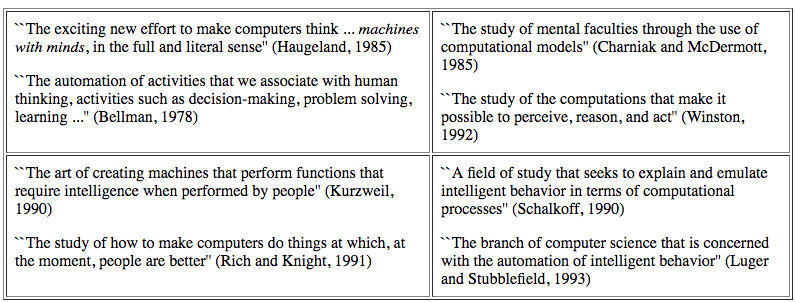
\includegraphics[width=\linewidth]{aidef}
    \caption{Possibili definizioni di Intelligenza artificiale}
    \label{fig:ai}
  \end{figure}
Dare un'unica definizione di intelligenza artificiale risulta estremamente difficile a causa della vastità
e dell'interdisciplinarietà dell'argomento. Soltanto nella figura \ref{fig:ai} troviamo otto possibili definizioni, ciascuna valida, ma
la descrizione  migliore per i nostri scopi  è quella data dal padre di questa disciplina John Mccarthy:
L'Intelligenza Artificiale è la scienza volta alla creazione di macchine  \emph{intelligenti},
più nello specifico di \emph{programmi intelligenti}.\cite{ai}

